% This must be in the first 5 lines to tell arXiv to use pdfLaTeX, which is strongly recommended.
\pdfoutput=1
% In particular, the hyperref package requires pdfLaTeX in order to break URLs across lines.

\documentclass[11pt]{article}

% Remove the "guidelines" option to generate the final version.
\usepackage[guidelines]{nlpreport} % show guidelines
%\usepackage[]{nlpreport} % hide guidelines


% Standard package includes
\usepackage{times}
\usepackage{latexsym}

% For proper rendering and hyphenation of words containing Latin characters (including in bib files)
\usepackage[T1]{fontenc}
% For Vietnamese characters
% \usepackage[T5]{fontenc}
% See https://www.latex-project.org/help/documentation/encguide.pdf for other character sets

% This assumes your files are encoded as UTF8
\usepackage[utf8]{inputenc}

% This is not strictly necessary, and may be commented out,
% but it will improve the layout of the manuscript,
% and will typically save some space.
\usepackage{microtype}
\usepackage{graphicx}
\usepackage{hyperref}
\usepackage{amsmath}
\usepackage{mathtools}
\usepackage{multirow}
\usepackage{listings}
\usepackage{xcolor}
\usepackage{booktabs} % for tables
\usepackage{multicol}
\usepackage{adjustbox}
\usepackage{float}
\usepackage{caption}
\usepackage{enumitem} % Package for customizing lists




% THE pdfinfo Title AND Author ARE NOT NECESSARY, THEY ARE METADATA FOR THE FINAL PDF FILE
\hypersetup{pdfinfo={
Title={Assignment 2},
Author={Federico Rullo}
}}
%\setcounter{secnumdepth}{0}  
 \begin{document}
%
\title{Assignment 2}
\author{Fabio Zanotti,
Antonio Morelli,
Federico Rullo
\and
Edoardo Conca\\
Master's Degree in Artificial Intelligence, University of Bologna\\
\{ fabio.zanotti, antonio.morelli, federico.rullo, edoardo.conca \}@studio.unibo.it
}
\maketitle

\begin{abstract}
%\begin{quote}

The experiment aimed to develop and evaluate models for a multi-label classification task on a dataset containing samples labeled with multiple categories. Three different model architectures were explored: CClassifier, CPClassifier, and CPSClassifier. Each model was trained and evaluated using per-category and macro F1-scores as performance metrics. Additionally, precision-recall curves were plotted to analyze the trade-off between precision and recall. The results showed that the CPSClassifier consistently outperformed the other models, demonstrating the effectiveness of incorporating additional input features for improved classification performance.

%\end{quote}
\end{abstract}

\section{Introduction}
\label{sec:introduction}
Multi-label classification tasks involve predicting multiple labels for each sample in a dataset. These tasks are prevalent in various domains, including natural language processing and healthcare. In this experiment, we developed and evaluated models for a multi-label classification task using a dataset containing samples labeled with psychological constructs. The objective was to predict these psychological construct labels based on text inputs. We explored three different model architectures: CClassifier, CPClassifier, and CPSClassifier, each incorporating different combinations of input features, based on BERT (Bidirectional Encoder Representations from Transformers), a state-of-the-art model in natural language processing, which serves as the backbone for our classification architectures due to its robust contextual understanding capabilities.The experiment aimed to assess the performance of these models using various evaluation metrics, including per-category and macro F1-scores, as well as precision-recall curves and a final comparison with a Random Uniform Classifier and a Majority Classifier.

\section{System description}
\label{sec:system}
The models evaluated in this study include:
\begin{itemize}
    \item BERT-based models - these models leverage pre-trained BERT architectures fine-tuned on our dataset. %Variants include:
    \item  Random Uniform Classifier - a baseline model that predicts classes uniformly at random.
    \item Majority Classifier: a baseline model that always predicts the most represented class in the dataset.
\end{itemize}
In the following list, the evaluated BERT model variants are described more precisely:
\begin{itemize}[label=$\diamond$]
    \item CClassifier: Basic BERT model for classification with conclusion text inputs \ref{fig:conclusion}.
    \item CPClassifier: BERT model incorporating both premise and conclusion text inputs \ref{fig:con_prem}.        \item CPSClassifier: BERT model that extends the previous models by incorporating premise, conclusion, and stance text inputs \ref{fig:con_prem_sta}.
\end{itemize}
We selected the tiny version of the BERT model, specifically the prajjwal1/bert-tiny, due to its lightweight nature, suitable for resource-constrained environments. We employ the AutoTokenizer to automatically load the tokenizer associated with the chosen model. Finally, we load the datasets using the DataLoader class, iterating through the dataset in batches of 16, with data shuffling enabled to ensure variability in each epoch.
\\From HuggingFace, we acknowledge that the maximum sequence length for our model is 512 tokens. The stance input is encoded into a numerical format, and the same model instance is used to encode both premise and conclusion inputs.
The models are then trained on the training dataset and evaluated on the validation set. Weighted loss functions are used to address class imbalance. 

\section{Experimental setup and results}
\label{sec:results}
\subsection{Parameter Tuning and Metrics}
To optimize model performance, we experimented with various learning rates (1e-3, 1e-5, 2e-5), batch sizes (8, 16, 32), training epochs (5, 10, 15), and weight decay values to prevent overfitting. Each parameter combination was evaluated on the validation set to find the optimal configuration.
\\Model performance was assessed using sklearn's f1\_score function. The average parameter allowed us to compute per-category binary F1-scores, while the macro parameter provided unweighted means across all labels, disregarding class imbalance.
\\Our data analysis revealed significant class imbalance. To address this, we calculated class weights based on the inverse frequency of each class, ensuring that under-represented classes received higher weights. This encouraged the model to focus more effectively on these classes by emphasizing their error during training.
\subsection{Results}
The experimental results highlight the critical role of incorporating additional input features, such as premise, conclusion, and stance, in improving model performance for multi-label classification tasks. The CPSClassifier, which integrates all three input features, demonstrated superior performance and emerged as the best-performing model on both validation and test sets.

\begin{table}[H]
\centering
\captionsetup{justification=centering, singlelinecheck=false}
\caption{F1 Scores on Validation Set}
\footnotesize
\begin{tabular}{|l|l|}
\hline
                                             & Macro F1 Scores \\ \hline
CClassifier                     & 0.679                  \\ \hline
CPClassifier                           & 0.73                   \\ \hline
CPSClassifier                     & \textbf{0.731}                  \\ \hline

\end{tabular}
\label{Tab:Tcr_1}
\end{table}

\begin{table}[H]
\centering
\captionsetup{justification=centering, singlelinecheck=false}
\caption{F1 Scores on Test Set}
\footnotesize
\begin{tabular}{|l|l|}
\hline
                                             & Macro F1 Scores \\ \hline
CClassifier                     & 0.610                  \\ \hline
CPClassifier                           & 0.692                   \\ \hline
CPSClassifier                     & \textbf{0.698}                  \\ \hline
Random Uniform Classifier                    & 0.503                  \\ \hline
Majority Classifier                    & 0.431                   \\ \hline
\end{tabular}
\label{Tab:Tcr_2}
\end{table}


\begin{table}[H]
\centering
\captionsetup{justification=centering, singlelinecheck=false}
\caption{F1 Scores on Test Set - CPSClassifier}
\footnotesize
\begin{tabular}{|l|l|}
\hline
                                            & Macro F1 Scores \\ \hline
Openness to change                     & 0.53                  \\ \hline
Self enhancement                         & 0.545                   \\ \hline
Conservation                     & 0.829                 \\ \hline
Self transcendence                     & 0.888                \\ \hline
Average                    & \textbf{0.698 }                  \\ \hline
\end{tabular}
\label{Tab:Tcr_3}
\end{table}



\section{Discussion}
\label{sec:discussion}
The similar performances between the CPSClassifier and the CPClassifier suggest that the slight improvement might be due to chance, confirming that stance values, being equally distributed, do not significantly enhance performance.
\\Moreover, correctly predicting "Openness to Change" and "Self-Enhancement," which are less represented classes, contributes highly to the overall score differences. This indicates that our models handle class imbalance effectively. 
\\In baseline comparisons, the BERT model consistently outperforms both the random and majority classifiers in precision, recall, and F1-score.This highlights the value of considering multiple contextual factors in text classification.
\\Analyzing the precision-recall curves provided insights into the models' trade-offs between precision and recall, emphasizing the challenges in balancing true positives and false positives. These curves illustrated how the CPSClassifier maintained a better balance compared to other models, showcasing its robustness in handling imbalanced datasets. While the CClassifier generally performs worse than the other two variants, tending to output similar predictions. When highly represented classes are true, the models rarely fail to predict correctly, underscoring the imbalance between positive and negative samples.

\section{Conclusion}
\label{sec:conclusion}
In conclusion, the experiment successfully developed and evaluated models for a multi-label classification task on a dataset containing samples labeled with psychological constructs. The CPSClassifier emerged as the best-performing model, demonstrating the importance of incorporating additional input features for improved classification performance. The experiment's findings suggest that fine-tuning model architectures and input features can significantly improve classification performance and offer deeper insights into the underlying data distribution and model behavior. The integration of various textual elements allows for a more comprehensive understanding and accurate classification, which is crucial for tasks that require detailed contextual analysis.

\section{Links to external resources}
\label{sec:links}
\href{https://github.com/antoniototimorelli/nlp_unibo_2023-24_assignments/tree/main/Assignment_2}{Assignment\_2}

\nocite{*}
\bibliography{nlpreport.bib}

\clearpage
\onecolumn 
\appendix
\section*{Appendix}
\subsection*{Figures}
\begin{figure}[H]
        \centering
        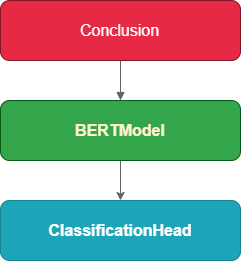
\includegraphics[scale=0.50]{img/C.png}
        \caption{CClassifier architecture}
        \label{fig:conclusion}
\end{figure}

%\vspace{50pt}
\begin{figure}[H]
        \centering
        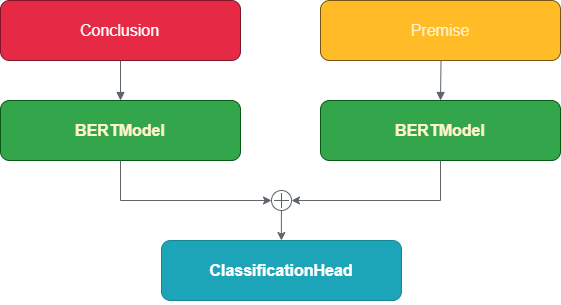
\includegraphics[scale=0.50]{img/CP.png}
        %\captionsetup{justification=raggedleft, singlelinecheck=false}
        \caption{CPClassifier architecture}
        \label{fig:con_prem}
\end{figure}

%\vspace{50pt}
\begin{figure}[H]
        \centering
        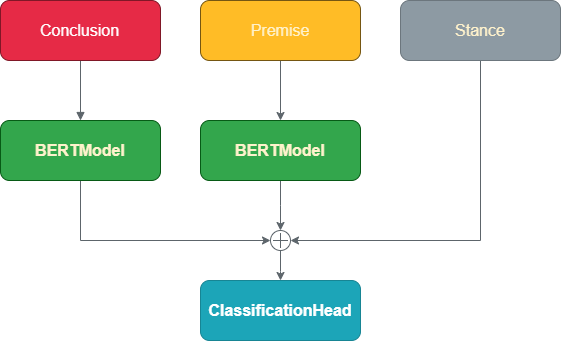
\includegraphics[scale=0.50]{img/CPS.png}
        \caption{CPSClassifier architecture}
        \label{fig:con_prem_sta}
\end{figure}

\end{document}

\begin{minipage}[t]{0.93\textwidth}
    \begin{figure}[H]
        \centering
        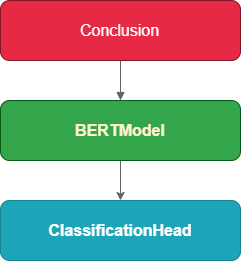
\includegraphics[scale=0.45]{img/C.png}
        \caption{CClassifier architecture}
        \label{fig:conclusion}
    \end{figure}
    \vspace{50pt}
    \begin{figure}[H]
        \centering
        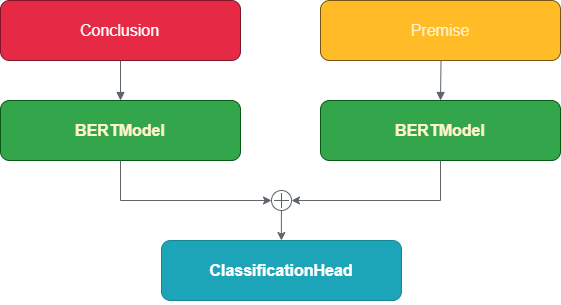
\includegraphics[scale=0.45]{img/CP.png}
        \caption{CPClassifier architecture}
        \captionsetup{justification=centering, singlelinecheck=false}
        \label{fig:con_prem}
    \end{figure}
    \vspace{50pt}
    \begin{figure}[H]
        \centering
        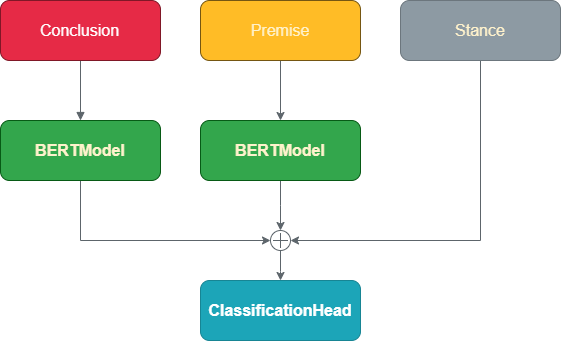
\includegraphics[scale=0.45]{img/CPS.png}
        \caption{CPSClassifier architecture}
        \label{fig:con_prem_sta}
    \end{figure}
    \end{minipage}

\begin{multicols}{2}

\begin{minipage}[t]{0.40\textwidth}
\section{Links to external resources}
\label{sec:links}
\href{https://github.com/antoniototimorelli/nlp_unibo_2023-24_assignments/tree/main/Assignment_2}{Assignment\_2}
\nocite{*}
\bibliography{nlpreport.bib}
\end{minipage}

\begin{minipage}[t]{0.93\textwidth}
    \begin{figure}[H]
        \centering
        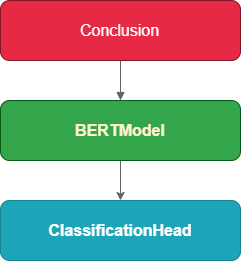
\includegraphics[scale=0.50]{img/C.png}
        \caption{CClassifier architecture}
        \label{fig:conclusion}
    \end{figure}
    \end{minipage}

\end{multicols}
\vspace{50pt}
\begin{figure}[H]
        \raggedleft
        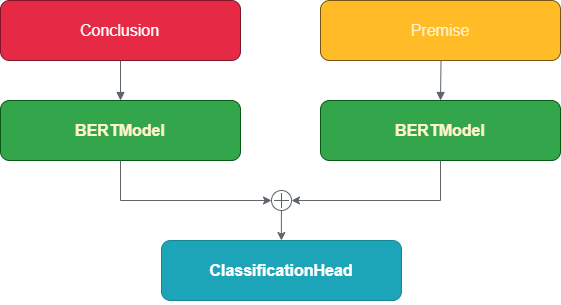
\includegraphics[scale=0.50]{img/CP.png}
        \caption{CPClassifier architecture}
        \label{fig:con_prem}
\end{figure}
\vspace{50pt}
\begin{figure}[H]
        \centering
        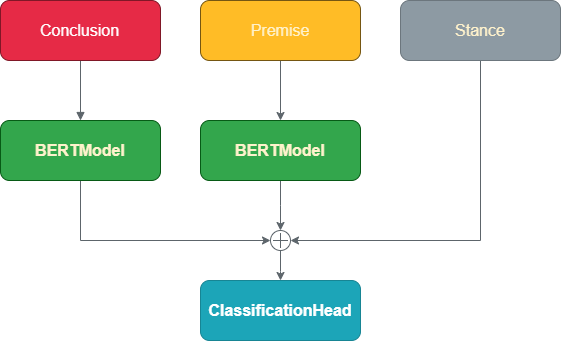
\includegraphics[scale=0.50]{img/CPS.png}
        \caption{CPSClassifier architecture}
        \label{fig:con_prem_sta}
\end{figure}

\begin{table}[ht]
\caption{Avg F1-score per category on validation set}
\footnotesize
\begin{tabular}{|l|l|l|l|l|}
\hline
& \textbf{CClassifier} & \textbf{CPClassifier} & \textbf{CPSClassifier} \\ \hline
O.C.  & 0.4            & \textbf{0.561}                 & 0.552         \\ \hline
S.E.  &0.572           & 0.632                 & \textbf{0.637}         \\ \hline
C.    & \textbf{0.859} & 0.854                 & 0.854                  \\ \hline
S.T.  & \textbf{0.885} & 0.873                 & 0.882                  \\ \hline 
\end{tabular}
\label{Tab:Tcr_1}
\end{table}